\PassOptionsToPackage{unicode=true}{hyperref} % options for packages loaded elsewhere
\PassOptionsToPackage{hyphens}{url}
\PassOptionsToPackage{dvipsnames,svgnames*,x11names*}{xcolor}
%
\documentclass[10pt,]{krantz}
\usepackage{lmodern}
\usepackage{amssymb,amsmath}
\usepackage{ifxetex,ifluatex}
\usepackage{fixltx2e} % provides \textsubscript
\ifnum 0\ifxetex 1\fi\ifluatex 1\fi=0 % if pdftex
  \usepackage[T1]{fontenc}
  \usepackage[utf8]{inputenc}
  \usepackage{textcomp} % provides euro and other symbols
\else % if luatex or xelatex
  \usepackage{unicode-math}
  \defaultfontfeatures{Ligatures=TeX,Scale=MatchLowercase}
    \setmonofont[Mapping=tex-ansi,Scale=0.7]{Source Code Pro}
\fi
% use upquote if available, for straight quotes in verbatim environments
\IfFileExists{upquote.sty}{\usepackage{upquote}}{}
% use microtype if available
\IfFileExists{microtype.sty}{%
\usepackage[]{microtype}
\UseMicrotypeSet[protrusion]{basicmath} % disable protrusion for tt fonts
}{}
\IfFileExists{parskip.sty}{%
\usepackage{parskip}
}{% else
\setlength{\parindent}{0pt}
\setlength{\parskip}{6pt plus 2pt minus 1pt}
}
\usepackage{xcolor}
\usepackage{hyperref}
\hypersetup{
            pdftitle={Elementos de la estadística},
            pdfauthor={Ricardo Michel MALLQUI BAÑOS},
            colorlinks=true,
            linkcolor=Maroon,
            filecolor=Maroon,
            citecolor=Blue,
            urlcolor=Blue,
            breaklinks=true}
\urlstyle{same}  % don't use monospace font for urls
\usepackage{longtable,booktabs}
% Fix footnotes in tables (requires footnote package)
\IfFileExists{footnote.sty}{\usepackage{footnote}\makesavenoteenv{longtable}}{}
\setlength{\emergencystretch}{3em}  % prevent overfull lines
\providecommand{\tightlist}{%
  \setlength{\itemsep}{0pt}\setlength{\parskip}{0pt}}
\setcounter{secnumdepth}{5}

% set default figure placement to htbp
\makeatletter
\def\fps@figure{htbp}
\makeatother

\usepackage[spanish,es-lcroman,es-tabla]{babel}
\usepackage{booktabs}
\usepackage{graphicx} 
\usepackage{amsmath}
\usepackage{makeidx}
\makeindex

\makeatletter\@addtoreset{chapter}{part}\makeatother%

%\usepackage{showframe}
%\usepackage[a4paper]{geometry}
%\geometry{verbose,tmargin=3cm,bmargin=3cm,lmargin=3.5cm,rmargin=3cm}
\renewcommand{\arraystretch}{1.1}

\usepackage{times}
\renewcommand{\rmdefault}{ptm}
\usepackage[lite,subscriptcorrection,nofontinfo,zswash]{mtpro2}

\usepackage{graphicx}

% Determine if the image is too wide for the page.
\makeatletter
\def\ScaleIfNeeded{%
  \ifdim\Gin@nat@width>\linewidth
    \linewidth
  \else
    \Gin@nat@width
  \fi
}
\makeatother

% Resize figures that are too wide for the page.
\let\oldincludegraphics\includegraphics
\renewcommand\includegraphics[2][]{%
  \oldincludegraphics[scale=0.85]{#2}
}

\usepackage{amsthm}
\makeatletter
\def\thm@space@setup{%
  \thm@preskip=8pt plus 2pt minus 4pt
  \thm@postskip=\thm@preskip
}
\makeatother



\flushbottom 

\frontmatter
\usepackage[]{natbib}
\bibliographystyle{apalike}

\title{Elementos de la estadística}
\providecommand{\subtitle}[1]{}
\subtitle{estadística descriptiva y probabilidades}
\author{Ricardo Michel MALLQUI BAÑOS}
\date{2020-04-06}

\usepackage{amsthm}
\newtheorem{theorem}{Teorema}[chapter]
\newtheorem{lemma}{Lema}[chapter]
\newtheorem{corollary}{Corolario}[chapter]
\newtheorem{proposition}{Proposición}[chapter]
\newtheorem{conjecture}{Conjectura}[chapter]
\theoremstyle{definition}
\newtheorem{definition}{Definición}[chapter]
\theoremstyle{definition}
\newtheorem{example}{Ejemplo}[chapter]
\theoremstyle{definition}
\newtheorem{exercise}{Ejercicio}[chapter]
\theoremstyle{remark}
\newtheorem*{remark}{Observación}
\newtheorem*{solution}{Solución}
\let\BeginKnitrBlock\begin \let\EndKnitrBlock\end
\begin{document}
\maketitle

%\cleardoublepage\newpage\thispagestyle{empty}\null
%\cleardoublepage\newpage\thispagestyle{empty}\null
%\cleardoublepage\newpage
\thispagestyle{empty}
\begin{center}
\includegraphics{U.pdf}
\end{center}

%\setlength{\abovedisplayskip}{-5pt}
%\setlength{\abovedisplayshortskip}{-5pt}

{
\hypersetup{linkcolor=}
\setcounter{tocdepth}{2}
\tableofcontents
}
\listoftables
\listoffigures
\newcommand{\N}{\mathbb{N}}
\newcommand{\R}{\mathbb{R}}
\newcommand{\CC}{\mathbb{C}}
\newcommand{\I}{\mathbb{I}}
\newcommand{\f}{\mathbb{f}}
\newcommand{\X}{\mathbb{X}}
\newcommand{\D}{\mathbb{D}}
\newcommand{\Z}{\mathbb{Z}}
\newcommand{\Q}{\mathbb{Q}}
\newcommand{\norm}[1]{\left\Vert#1\right\Vert}
\newcommand{\abs}[1]{\left\vert#1\right\vert}
\newcommand{\set}[1]{\left\{#1\right\}}
\newcommand{\seq}[1]{\left<#1\right>}
\newcommand{\co}[1]{\left[#1\right]}
\newcommand{\cc}[1]{\left(#1\right)}
\newcommand{\J}{\mathcal{J}}
\newcommand{\K}{\mathcal{K}}
\newcommand{\M}{\mathcal{M}}
\newcommand{\F}{\mathcal{F}}

\hypertarget{resumen}{%
\chapter*{Resumen}\label{resumen}}


La estadística es la ciencia que manipula datos las analiza e interpreta para poder sacar concluciones razonables de ciertos fenomenos naturales. Esta ciencia puede ser dividido en dos: \textbf{estadística descirptiva} y \textbf{estadística inferencial}. En la estadística descriptiva se procesan datos de una manera teórica y utilitaria. Estos métodos consisten en la recolección, organización, resumen, descripcion y presenatacion de la información. Si la poblacion está disponible entonces la estadística descriptiva es suficiente para describir ciertos fenomenos. No obstante generalmente no se dispone de toda la población si no de una muestra de ella, es en este caso que se requieren usar técnicas más sofisticadas para tomar decisiones y generalizaciones acerca de la poblacion, desde una pequeña muestra de información. Es cuando entra en el juego la estadística inferencial.

La base teórica de la estadística son las matemáticas

Este libro se compone de dos partes, la primera parte trata sobre la \textbf{estadística descirptiva} y la segunda \textbf{estadística inferencial}. Cada una de ellas divididas en capítulos.

\mainmatter

\hypertarget{part-estaduxedstica-descriptiva}{%
\part{Estadística descriptiva}\label{part-estaduxedstica-descriptiva}}

\hypertarget{prerrequisitos}{%
\chapter{Prerrequisitos}\label{prerrequisitos}}

\hypertarget{variables}{%
\chapter{Variables}\label{variables}}

Es una característica de personas cosas u objetos que sonpropensos a ser medidas
\#\# Variables cualitativas

Denotan cualidades de objetos personas o animales tales como caracteristicas inherentes que no son medibles por números, tenemos dos casos de esta variable.

\hypertarget{nominales}{%
\subsection{Nominales}\label{nominales}}

Son caracteristicas que simplemente nominan y estan propensos a ser jerarquizados u ordenados tales como: El estado civil (soltero, casado, divorciado, viudo), Religion (católic, evangelico, judio, etc).\#

\hypertarget{ordinales}{%
\subsection{Ordinales}\label{ordinales}}

Son caracteristicas que que si están propensos a ser jerarquizados tales como: Nivel de instrucción (primaria, secundaria, superior).

\hypertarget{variables-cuantitativas}{%
\section{Variables cuantitativas}\label{variables-cuantitativas}}

Son aqueelllas variables que están propensos a ser medidas mediante números ya sean números enteros o reales.

\hypertarget{discretas}{%
\subsection{Discretas}\label{discretas}}

Aquellas que solo son medidos mediante numeros enteros por ejemplo: Número de hijos, número de habitaciones.

\hypertarget{continuas}{%
\subsection{Continuas}\label{continuas}}

Aquellas que solo son medidos mediante numeros reales es decir este incluye a los numeros racionales e irracionales. Estatura, volumen, peso.

\hypertarget{caracteruxedstica-de-los-datos}{%
\chapter{Característica de los datos}\label{caracteruxedstica-de-los-datos}}

\hypertarget{poblaciuxf3n-muestra-y-estaduxedstica}{%
\chapter{Población, muestra y estadística}\label{poblaciuxf3n-muestra-y-estaduxedstica}}

\hypertarget{organizaciuxf3n-de-datos-en-tablas-de-frecuencias}{%
\chapter{Organización de datos en tablas de frecuencias}\label{organizaciuxf3n-de-datos-en-tablas-de-frecuencias}}

\begin{verbatim}
## [1] 0.9500042
\end{verbatim}

\begin{verbatim}
## [1] 1
\end{verbatim}

\begin{figure}

{\centering 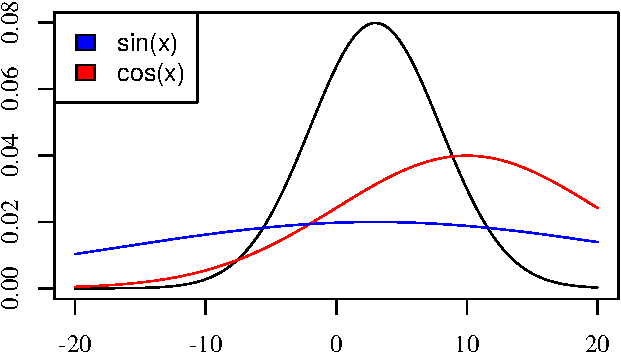
\includegraphics{E_1_files/figure-latex/99w-1} 

}

\caption{Regresión lineal}\label{fig:99w1}
\end{figure}
\begin{figure}

{\centering 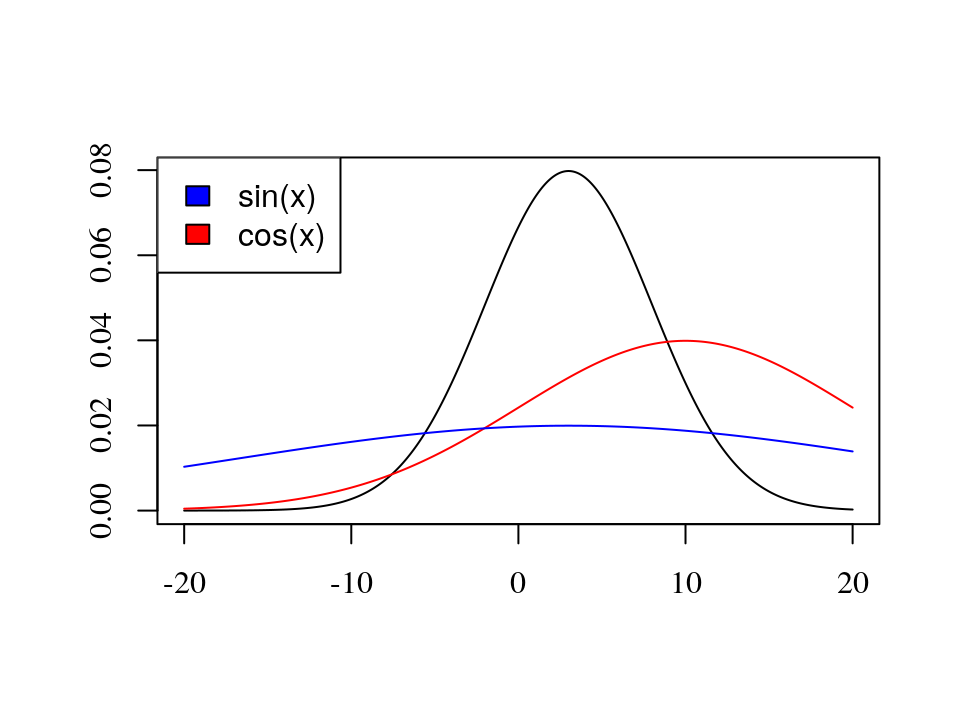
\includegraphics{E_1_files/figure-latex/99w-2} 

}

\caption{Regresión lineal}\label{fig:99w2}
\end{figure}

\[\frac{1}{x^2}=1\]

\[\frac{\sin x}{x^3}=0.3794281\]

\[\Phi_{\mu ,\sigma ^{2}}(x)=\frac {1}{\sigma {\sqrt {2\pi }}}e^{-{\frac {(u-\mu )^{2}}{2\sigma ^{2}}}}du\]

\begin{itemize}
\tightlist
\item
  \[\frac{1}{20\sqrt{2\pi }}\int_{-\infty }^{ 300}e^{- \frac{1}{2}\left(\frac{z-200}{20}\right)^2}dz=0.9999997\]
\item
  0.9500042 also Es decir los elementos son demagogos y déspotas
\item
  Es decir los elementos son demagogos y déspotas
  Tabla \ref{tab:ww1}
\end{itemize}

\begin{longtable}[]{@{}rclrl@{}}
\caption{\label{tab:ww1} Caption}\tabularnewline
\toprule
\begin{minipage}[b]{0.26\columnwidth}\raggedleft
Option\strut
\end{minipage} & \begin{minipage}[b]{0.08\columnwidth}\centering
N\strut
\end{minipage} & \begin{minipage}[b]{0.03\columnwidth}\raggedright
w\strut
\end{minipage} & \begin{minipage}[b]{0.23\columnwidth}\raggedleft
Observation\strut
\end{minipage} & \begin{minipage}[b]{0.26\columnwidth}\raggedright
Description\strut
\end{minipage}\tabularnewline
\midrule
\endfirsthead
\toprule
\begin{minipage}[b]{0.26\columnwidth}\raggedleft
Option\strut
\end{minipage} & \begin{minipage}[b]{0.08\columnwidth}\centering
N\strut
\end{minipage} & \begin{minipage}[b]{0.03\columnwidth}\raggedright
w\strut
\end{minipage} & \begin{minipage}[b]{0.23\columnwidth}\raggedleft
Observation\strut
\end{minipage} & \begin{minipage}[b]{0.26\columnwidth}\raggedright
Description\strut
\end{minipage}\tabularnewline
\midrule
\endhead
\begin{minipage}[t]{0.26\columnwidth}\raggedleft
Es decir los elementos son demagogos y déspotas Es decir los elementos son demagogos y déspotas\strut
\end{minipage} & \begin{minipage}[t]{0.08\columnwidth}\centering
1\strut
\end{minipage} & \begin{minipage}[t]{0.03\columnwidth}\raggedright
w\strut
\end{minipage} & \begin{minipage}[t]{0.23\columnwidth}\raggedleft
Es decir los elementos son demagogos y déspotas\strut
\end{minipage} & \begin{minipage}[t]{0.26\columnwidth}\raggedright
Es decir los elementos son demagogos y déspotas Es decir los elementos son demagogos y déspotas\strut
\end{minipage}\tabularnewline
\begin{minipage}[t]{0.26\columnwidth}\raggedleft
Engine\strut
\end{minipage} & \begin{minipage}[t]{0.08\columnwidth}\centering
2\strut
\end{minipage} & \begin{minipage}[t]{0.03\columnwidth}\raggedright
w\strut
\end{minipage} & \begin{minipage}[t]{0.23\columnwidth}\raggedleft
Es decir los elementos son demagogos y déspotas \(\sum^{n}_{i=1}{f_i}\)\strut
\end{minipage} & \begin{minipage}[t]{0.26\columnwidth}\raggedright
Engine to be used for processing templates. Handlebars is the default.\strut
\end{minipage}\tabularnewline
\begin{minipage}[t]{0.26\columnwidth}\raggedleft
Es decir los elementos son demagogos y déspotas\strut
\end{minipage} & \begin{minipage}[t]{0.08\columnwidth}\centering
3\strut
\end{minipage} & \begin{minipage}[t]{0.03\columnwidth}\raggedright
w\strut
\end{minipage} & \begin{minipage}[t]{0.23\columnwidth}\raggedleft
\(\sum^{n}_{i=1}{f_i}\)\strut
\end{minipage} & \begin{minipage}[t]{0.26\columnwidth}\raggedright
extension to be used for dest files.\strut
\end{minipage}\tabularnewline
\bottomrule
\end{longtable}

variable aleatoria Variable aleatoria entonces

2.7182818 0.9750021 0.7881446

2

The value of \texttt{x} in the Python session is Es decir los elementos son demagogos y déspotas.
It is not the same \texttt{x} as the one in R.

\begin{verbatim}
## Nonlinear regression model
##   model: y ~ a + b * I(x^z)
##    data: parent.frame()
##        a        b        z 
## 30.83221  0.01163  3.51762 
##  residual sum-of-squares: 106851
## 
## Number of iterations to convergence: 23 
## Achieved convergence tolerance: 3.462e-06
\end{verbatim}

\begin{figure}

{\centering 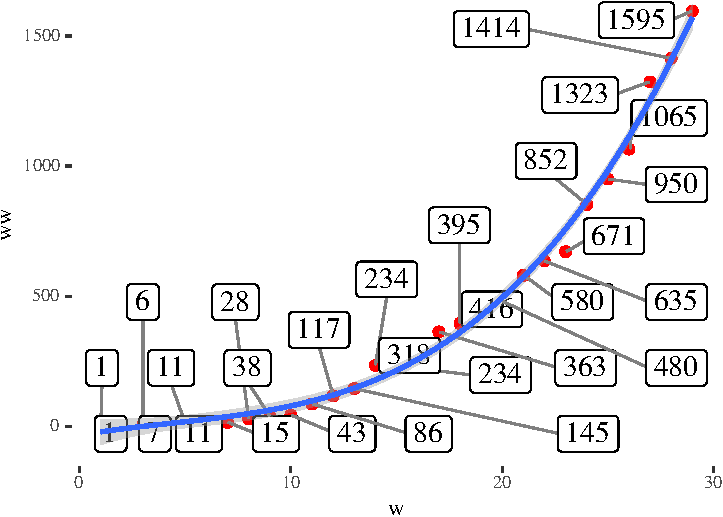
\includegraphics{E_1_files/figure-latex/ww1w-1} 

}

\caption{Regresión lineal}\label{fig:ww1w1}
\end{figure}

\begin{verbatim}
## [1] 76088.81
\end{verbatim}

\begin{figure}

{\centering 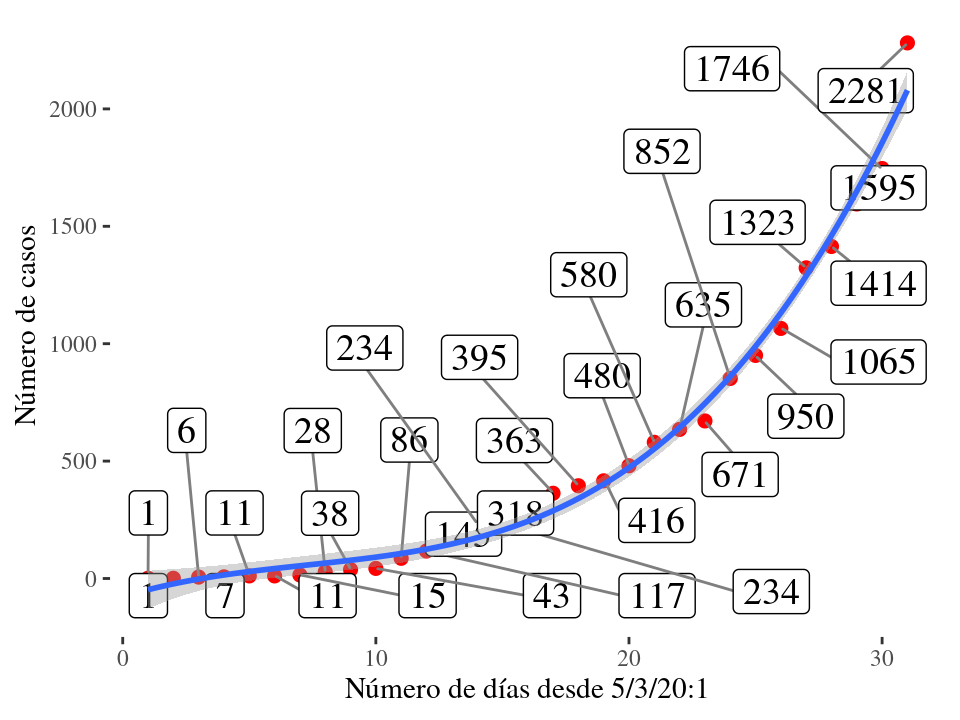
\includegraphics{E_1_files/figure-latex/ww1w-2} 

}

\caption{Regresión lineal}\label{fig:ww1w2}
\end{figure}

\[f(x)=-77.602+32.606x+-2.892x^2+0.132x^3\]

\begin{longtable}[]{@{}ccc@{}}
\toprule
\endhead
\begin{minipage}[t]{0.28\columnwidth}\centering
\(f(30)_{\text{04 abril}}=1856\)\strut
\end{minipage} & \begin{minipage}[t]{0.33\columnwidth}\centering
\(f(31)_{\text{05 abril}}=2080\)\strut
\end{minipage} & \begin{minipage}[t]{0.30\columnwidth}\centering
\(f(32)=2322\)\strut
\end{minipage}\tabularnewline
\begin{minipage}[t]{0.28\columnwidth}\centering
\(f(33)=2584\)\strut
\end{minipage} & \begin{minipage}[t]{0.33\columnwidth}\centering
\(f(34)=2867\)\strut
\end{minipage} & \begin{minipage}[t]{0.30\columnwidth}\centering
\(f(35)=3171\)\strut
\end{minipage}\tabularnewline
\begin{minipage}[t]{0.28\columnwidth}\centering
\(f(36)=3496\)\strut
\end{minipage} & \begin{minipage}[t]{0.33\columnwidth}\centering
\(f(37)=3844\)\strut
\end{minipage} & \begin{minipage}[t]{0.30\columnwidth}\centering
\(f(38)=4216\)\strut
\end{minipage}\tabularnewline
\begin{minipage}[t]{0.28\columnwidth}\centering
\textbf{\(f(39)_{\text{-}}=4612\)}\strut
\end{minipage} & \begin{minipage}[t]{0.33\columnwidth}\centering
\(f(40)=5033\)\strut
\end{minipage} & \begin{minipage}[t]{0.30\columnwidth}\centering
\(f(41)=5480\)\strut
\end{minipage}\tabularnewline
\begin{minipage}[t]{0.28\columnwidth}\centering
\(f(100)=\ensuremath{1.06036\times 10^{5}}\)\strut
\end{minipage} & \begin{minipage}[t]{0.33\columnwidth}\centering
\(f(360)=\ensuremath{5.784933\times 10^{6}}\)\strut
\end{minipage} & \begin{minipage}[t]{0.30\columnwidth}\centering
\(f(370)=\ensuremath{6.290851\times 10^{6}}\)\strut
\end{minipage}\tabularnewline
\bottomrule
\end{longtable}

Sea la Tabla \ref{tab:2w3} Figures and tables with captions will be placed in \texttt{figure} and \texttt{table} environments, respectively.

\begin{longtable}[t]{cccccccccc}
\caption{\label{tab:2w3}Figures and tables with captions will be placed in `figure`}\\
\toprule
$Y_i$ & $f_i$ & $F_i$ & $F_i^*$ & $h_i$ & $H_i$ & $H_i^*$ & $h_i\%$ & $H_i\%$ & $H_i^*\%$\\
\midrule
a & 1 & 1 & 73 & 0.01 & 0.01 & 1.00 & 1.37 & 1.37 & 100.00\\
b & 2 & 3 & 72 & 0.03 & 0.04 & 0.99 & 2.74 & 4.11 & 98.63\\
c & 3 & 6 & 70 & 0.04 & 0.08 & 0.96 & 4.11 & 8.22 & 95.89\\
d & 4 & 10 & 67 & 0.05 & 0.14 & 0.92 & 5.48 & 13.70 & 91.78\\
e & 5 & 15 & 63 & 0.07 & 0.21 & 0.86 & 6.85 & 20.55 & 86.30\\
f & 6 & 21 & 58 & 0.08 & 0.29 & 0.79 & 8.22 & 28.77 & 79.45\\
g & 7 & 28 & 52 & 0.10 & 0.38 & 0.71 & 9.59 & 38.36 & 71.23\\
h & 8 & 36 & 45 & 0.11 & 0.49 & 0.62 & 10.96 & 49.32 & 61.64\\
i & 9 & 45 & 37 & 0.12 & 0.62 & 0.51 & 12.33 & 61.64 & 50.68\\
j & 10 & 55 & 28 & 0.14 & 0.75 & 0.38 & 13.70 & 75.34 & 38.36\\
k & 6 & 61 & 18 & 0.08 & 0.84 & 0.25 & 8.22 & 83.56 & 24.66\\
l & 5 & 66 & 12 & 0.07 & 0.90 & 0.16 & 6.85 & 90.41 & 16.44\\
m & 3 & 69 & 7 & 0.04 & 0.95 & 0.10 & 4.11 & 94.52 & 9.59\\
n & 2 & 71 & 4 & 0.03 & 0.97 & 0.05 & 2.74 & 97.26 & 5.48\\
ñ & 1 & 72 & 2 & 0.01 & 0.99 & 0.03 & 1.37 & 98.63 & 2.74\\
o & 1 & 73 & 1 & 0.01 & 1.00 & 0.01 & 1.37 & 100.00 & 1.37\\
$\sum_{i=1}^6$ & 73 &  &  & 1.00 &  &  &  &  & \\
\bottomrule
\end{longtable}

\begin{longtable}[t]{lrllllll}
\caption{\label{tab:unnamed-chunk-1}Figures and tables with captions will be placed in `figure`}\\
\toprule
  & $\overline{x}$ & $\alpha$ & $\sum^{n}_{i=1}{x_i}$ & $\overline{x}$ & $\overline{x}$ & $\overline{x}$ & X7\\
\midrule
1 &  & IT1 & IT2 & O1 & IT3 & IT4 & IT5\\
2 & 1 & 2 & 2 & 2 & 2 & 1 & 1\\
3 & 2 & 3 & 2 & 3 & 3 & 3 & 3\\
4 & 3 & 3 & 3 & 3 & 3 & 2 & 2\\
5 & 4 & 3 & 3 & 3 & 2 & 2 & 2\\
6 & 5 & 3 & 2 & 3 & 3 & 3 & 3\\
$\beta_0$ & 6 & 1 & 1 & 1 & 1 & 2 & 2\\
$\beta_1$ & 7 & 2 & 3 & 3 & 3 & 3 & 2\\
$\beta_3$ & 8 & 2 & 2 & 2 & 1 & 1 & 1\\
10 & 9 & 1 & 2 & 2 & 1 & 1 & 1\\
11 & 10 & 1 & 2 & 2 & 2 & 1 & 1\\
12 & 11 & 2 & 2 & 2 & 2 & 2 & 2\\
13 & 12 & 2 & 3 & 3 & 3 & 2 & 2\\
14 & 13 & 3 & 2 & 3 & 3 & 2 & 2\\
15 & 14 & 2 & 3 & 3 & 2 & 2 & 3\\
16 & 15 & 2 & 2 & 2 & 2 & 2 & 1\\
17 & 16 & 2 & 2 & 2 & 3 & 2 & 3\\
18 & 17 & 2 & 2 & 2 & 2 & 2 & 2\\
19 & 18 & 1 & 2 & 2 & 1 & 1 & 2\\
20 & 19 & 3 & 2 & 3 & 3 & 3 & 3\\
21 & 20 & 3 & 3 & 3 & 3 & 2 & 2\\
22 & 21 & 1 & 1 & 1 & 1 & 2 & 2\\
23 & 22 & 3 & 3 & 3 & 3 & 3 & 2\\
24 & 23 & 3 & 2 & 3 & 3 & 3 & 3\\
25 & 24 & 3 & 2 & 3 & 3 & 3 & 3\\
26 & 25 & 2 & 3 & 3 & 3 & 3 & 2\\
27 & 26 & 2 & 2 & 2 & 1 & 1 & 1\\
28 & 27 & 1 & 2 & 2 & 1 & 2 & 2\\
29 & 28 & 3 & 2 & 3 & 3 & 2 & 2\\
30 & 29 & 3 & 2 & 3 & 3 & 3 & 3\\
31 & 30 & 1 & 2 & 2 & 2 & 1 & 1\\
32 & 31 & 3 & 3 & 3 & 3 & 3 & 2\\
33 & 32 & 3 & 3 & 3 & 2 & 3 & 3\\
34 & 33 & 1 & 1 & 1 & 1 & 1 & 1\\
$\sum^{n}_{i=1}{x_i}$ & 34 & 1 & 1 & 1 & 1 & 1 & 1\\
36 & 35 & 3 & 2 & 3 & 2 & 2 & 2\\
37 &  & $\sum_{i=1}^nx_i$ &  &  &  &  & \\
\bottomrule
\end{longtable}

\hypertarget{distribuciuxf3n-de-frecuencias}{%
\chapter{Distribución de frecuencias}\label{distribuciuxf3n-de-frecuencias}}

La tabulación es un proceso en el cual los datos son ordenados en grupos llamados \emph{clases} para un análisis más eficaz de estos, los datos podrían estar clasificados mediante una variable cualitativa o cuantitativa en el caso de las variables cualitativas \(Y_i\), se considera la siguiente Tabla \ref{tab:ww}

\begin{longtable}[]{@{}cccccccccc@{}}
\caption{\label{tab:ww} Caption}\tabularnewline
\toprule
\(Y_i\) & \(f_i\) & \(F_i\) & \(F_i^*\) & \(h_i\) & \(H_i\) & \(H_i^*\) & \(h_i\%\) & \(H_i\%\) & \(H_i^*\%\)\tabularnewline
\midrule
\endfirsthead
\toprule
\(Y_i\) & \(f_i\) & \(F_i\) & \(F_i^*\) & \(h_i\) & \(H_i\) & \(H_i^*\) & \(h_i\%\) & \(H_i\%\) & \(H_i^*\%\)\tabularnewline
\midrule
\endhead
\(Y_1\) & \(f_1\) & \(F_1\) & \(F_1^*\) & \(\frac{f_1}{n}\) & \(\frac{F_1}{n}\) & \(\frac{F_1^*}{n}\) & \(h_1\) & \(H_1\) & \(H_1^*\)\tabularnewline
\(Y_2\) & \(f_2\) & \(F_2\) & \(F_2^*\) & \(\frac{f_2}{n}\) & \(\frac{F_2}{n}\) & \(\frac{F_2^*}{n}\) & \(h_2\) & \(H_2\) & \(H_1^*\)\tabularnewline
\(Y_3\) & \(f_3\) & \(F_3\) & \(F_3^*\) & \(\frac{f_3}{n}\) & \(\frac{F_3}{n}\) & \(\frac{F_3^*}{n}\) & \(h_3\) & \(H_3\) & \(H_1^*\)\tabularnewline
\(\vdots\) & \(\vdots\) & \(\vdots\) & \(\vdots\) & \(\vdots\) & \(\vdots\) & \(\vdots\) & \(\vdots\) & \(\vdots\) & \(\vdots\)\tabularnewline
\(Y_r\) & \(f_r\) & \(F_r\) & \(F_r^*\) & \(\frac{f_r}{n}\) & \(\frac{F_r}{n}\) & \(\frac{F_r^*}{n}\) & \(h_r\) & \(H_r\) & \(H_1^*\)\tabularnewline
\bottomrule
\end{longtable}

En el caso de variables cuantitativas ademas si los datos son muy variados, que para se clasificados adecuadamente, necesitan generarse particiones de longitudes semejantes entonces se utiliza el siguiente proceso; el \textbf{número de las particiones} \(r\) se consideran de acuerdo a \textbf{tres criterios}

\begin{enumerate}
\def\labelenumi{\arabic{enumi}.}
\item
  Criterio del investigador \(r\) no puede ser más de 20 ni menos de 5
\item
  \(r=\sqrt{n}\) donde \(n\) es el número de datos
\item
  La regla de Starges que consiste en considerar la fórmula \(r=3.322\cdot\log_{10} n\)
  Una vez establecido el número de particiones se procede a generar los límites laterales de cada una de las particiones, sea \(L\) la longitud de todo el conjunto es decir \(L=x_{\text{max}}-x_{\text{min}}\) entonces la longitud de las particiones o amplitud interválica se obtiene con \(l=\frac{L}{r}\)
\end{enumerate}

\begin{longtable}[]{@{}ccccccccc@{}}
\toprule
Clase & Clase & \(f_i\) & \(F_i\) & \(F_i^*\) & \(h_i\) & \(H_i\) & \(H_i^*\) & \(\ldots\)\tabularnewline
\midrule
\endhead
\([y_1-y_2>\) & \(y_1\) & \(f_1\) & \(F_1\) & \(F_1^*\) & \(\frac{f_1}{n}\) & \(\frac{F_1}{n}\) & \(\frac{F_1^*}{n}\) & \(\ldots\)\tabularnewline
\(<y_1-y_2>\) & \(y_2\) & \(f_2\) & \(F_2\) & \(F_2^*\) & \(\frac{f_2}{n}\) & \(\frac{F_2}{n}\) & \(\frac{F_2^*}{n}\) & \(\ldots\)\tabularnewline
\(<y_{r}-y_r>\) & \(y_3\) & \(f_3\) & \(F_3\) & \(F_3^*\) & \(\frac{f_3}{n}\) & \(\frac{F_3}{n}\) & \(\frac{F_3^*}{n}\) & \(\ldots\)\tabularnewline
\(\vdots\) & \(\vdots\) & \(\vdots\) & \(\vdots\) & \(\vdots\) & \(\vdots\) & \(\vdots\) & \(\vdots\) & \(\vdots\)\tabularnewline
\(<y_{r-1}-y_r]\) & \(y_r\) & \(f_r\) & \(F_r\) & \(F_r^*\) & \(\frac{f_r}{n}\) & \(\frac{F_r}{n}\) & \(\frac{F_r^*}{n}\) & \(...\)\tabularnewline
\bottomrule
\end{longtable}

Tenga en cuenta que \(n\) es el número de datos, es decir \(n=f_1+f_2+\ldots+f_r=\sum_{i=1}^r\) donde \(f_i\) es número de datos en la partición \(X_i\), una de las \(r\) particiones del conjunto total de datos.

\begin{enumerate}
\def\labelenumi{\arabic{enumi}.}
\item
  Las \textbf{frecuencias absolutas}\index{frecuencias absolutas} \(f_i\) indican el número de datos con la característica \(X_i\).
\item
  Las \textbf{frecuencias absolutas acumuladas menor que}\index{frecuencias absolutas acumuladas menor que} \(F_i\) obedecen a la fórmula
  \[F_m=f_1+f_2+\ldots+f_m=\sum_{i=1}^mf_i\]
\item
  Las \textbf{frecuencias absolutas acumuladas mayor que} \(F_i^*\) obedecen a la fórmula
  \[F_m^*=f_m+f_{m+1}+\ldots+f_r=\sum_{i=m}^rf_i=n-\sum_{i=1}^{m-1}f_i=n-\left(f_1+f_{2}+\ldots+f_{m-1}\right)\]
\item
  Las \textbf{frecuencias absolutas relativas}\index{frecuencias absolutas relativas} obedecen a la fórmula
  \[h_m=\frac{f_m}{n}\]
\item
  Las \textbf{frecuencias absolutas relativas menor que}\index{frecuencias absolutas relativas  menor que} obedecen a la fórmula
  \[H_m=\frac{f_m}{n}\]
\item
  Las \textbf{frecuencias absolutas relativas mayor que} obedecen a la fórmula
  \[H_m^*=\frac{F_m}{n}\]
\item
  Las \textbf{frecuencias absolutas relativas porcentuales} obedecen a la fórmula
  \(h_i\%=100\cdot h_i\)
\item
  Las \textbf{frecuencias absolutas relativas menor que porcentuales} obedecen a la fórmula
  \(H_i\%=100\cdot H_i\)
\item
  Las \textbf{frecuencias absolutas relativas mayor que porcentuales} obedecen a la fórmula
  \(H_i^*\%=100\cdot H_i^*\)
\end{enumerate}

\BeginKnitrBlock{exercise}
\protect\hypertarget{exr:unnamed-chunk-2}{}{\label{exr:unnamed-chunk-2} }Sean los datos
\EndKnitrBlock{exercise}

\BeginKnitrBlock{solution}
\iffalse{} {Solución. } \fi{}Entonces
\EndKnitrBlock{solution}

\hypertarget{gruxe1ficos-estaduxedsticos}{%
\chapter{Gráficos estadísticos}\label{gruxe1ficos-estaduxedsticos}}

The value of \texttt{x} in the Python session is Es decir los elementos son demagogos y déspotas.
It is not the same \texttt{x} as the one in R.

\hypertarget{medidas-de-tendencia-central}{%
\chapter{Medidas de tendencia central}\label{medidas-de-tendencia-central}}

Son aquellas medidas que buscan un dato representtivo central de un conjunto de datos tales como la media, la moda y la mediana.

\hypertarget{la-media-overlinex}{%
\section{\texorpdfstring{La media (\(\overline{x}\))}{La media (\textbackslash{}overline\{x\})}}\label{la-media-overlinex}}

A veces llamada \emph{promedio aritmético}, es la medida de tendencia central que pondera los datos.

\hypertarget{media-de-datos-no-agrupados}{%
\subsection{Media de datos no agrupados}\label{media-de-datos-no-agrupados}}

Los datos no están agrupados cuando no están ordenados sobre una tabla de distribución de frecuencias. Sean los \(n\) datos \(x_1, x_2,\ldots, x_n\) entonces la media o promedio aritmético se define como
\begin{equation}
\overline{x}=\frac{x_1+x_2+\cdots+x_n}{n}=\frac{1}{n}\sum_{i=1}^nx_i
\label{eq:w1}
\end{equation}
\begin{equation}
\frac{d\left[P;F_1\right]}{d\left[P;\mathcal{L}_1\right]}=e=\frac{d\left[P;F_2\right]}{d\left[P;\mathcal{L}_2\right]}
\label{eq:ww}
\end{equation}

\begin{enumerate}
\def\labelenumi{\arabic{enumi}.}
\tightlist
\item
  \(\overline{x}=\frac{x_1+x_2+\cdots+x_n}{n}=\frac{1}{n}\sum_{i=1}^nx_i\)
\item
  \(\overline{x}=\frac{x_1+x_2+\cdots+x_n}{n}=\frac{1}{n}\sum_{i=1}^nx_i\)
\end{enumerate}

\hypertarget{media-de-datos-agrupados}{%
\subsection{Media de datos agrupados}\label{media-de-datos-agrupados}}

Considérese la siguiente tabla de distribucion de frecuencias entonces el promedio es \[\overline{x}=\frac{y_1f_1+y_2f_2+\cdots+y_nf_n}{n}=\frac{1}{n}\sum_{i=1}^ny_if_i\]

\begin{longtable}[]{@{}ccccccccc@{}}
\toprule
Clase & Clase & \(f_i\) & \(F_i\) & \(F_i^*\) & \(h_i\) & \(H_i\) & \(H_i^*\) & \(\ldots\)\tabularnewline
\midrule
\endhead
\(<y_1-y_2>\) & \(y_1\) & \(f_1\) & \(F_1\) & \(F_1^*\) & \(\frac{f_1}{n}\) & \(\frac{F_1}{n}\) & \(\frac{F_1^*}{n}\) & \(\ldots\)\tabularnewline
\(<y_2-y_3>\) & \(y_2\) & \(f_2\) & \(F_2\) & \(F_2^*\) & \(\frac{f_2}{n}\) & \(\frac{F_2}{n}\) & \(\frac{F_2^*}{n}\) & \(\ldots\)\tabularnewline
\(<y_3-y_4>\) & \(y_3\) & \(f_3\) & \(F_3\) & \(F_3^*\) & \(\frac{f_3}{n}\) & \(\frac{F_3}{n}\) & \(\frac{F_3^*}{n}\) & \(\ldots\)\tabularnewline
\(\vdots\) & \(\vdots\) & \(\vdots\) & \(\vdots\) & \(\vdots\) & \(\vdots\) & \(\vdots\) & \(\vdots\) & \(\vdots\)\tabularnewline
\(<y_{r-1}-y_r]\) & \(y_r\) & \(f_r\) & \(F_r\) & \(F_r^*\) & \(\frac{f_r}{n}\) & \(\frac{F_r}{n}\) & \(\frac{F_r^*}{n}\) & \(...\)\tabularnewline
\bottomrule
\end{longtable}

\BeginKnitrBlock{exercise}
\protect\hypertarget{exr:unnamed-chunk-4}{}{\label{exr:unnamed-chunk-4} }Si el promedio de \(n\) datos es \(\overline{x}\) entonces el promedio del conjunto inicial más un dato adicional \(x_{n+1}\) es \[\overline{x}'=\frac{n\overline{x}+x_{n+1}}{n+1}\] en general si se adicionan \(r\) datos \(y_1, y_2, \ldots y_r\) entonces el nuevo promedio será \[\overline{x}'=\frac{n\overline{x}+y_{1}+y_2+\ldots+y_r}{n+r}\]
\EndKnitrBlock{exercise}

\BeginKnitrBlock{solution}
\iffalse{} {Solución. } \fi{}En efecto sea el promedio
\begin{align*}
\overline{x}'&=\frac{x_1+x_2+\cdots+x_{n+1}}{n+1}\\
&=\frac{n\frac{x_1+x_2+\cdots x_n}{n}+x_{n+1}}{n+1}\\
&=\frac{n\overline{x}+x_{n+1}}{n+1}
\end{align*}
\EndKnitrBlock{solution}

\hypertarget{la-moda-mo}{%
\section{La moda (Mo)}\label{la-moda-mo}}

\hypertarget{moda-de-datos-no-tabulados}{%
\subsection{Moda de datos no tabulados}\label{moda-de-datos-no-tabulados}}

En este caso es dato que más repite en un conjunto de datos dados.

La moda es el dato que más se repite por ejemplo sea el conjunto de datos \(x_1,\) \(x_2,\) \(x_2,\) \(x_2,\) \(x_3\) entonces la moda \(\text{Mo}=x_2\)

\hypertarget{moda-de-datos-tabulados}{%
\subsection{Moda de datos tabulados}\label{moda-de-datos-tabulados}}

La moda es el dato que más se repite por ejemplo sea el conjunto de datos \(x_1,\) \(x_2,\) \(x_2,\) \(x_2,\) \(x_3\) entonces la moda \(\text{Mo}=Li+\frac{Li-Ls}{Li+Ls}r\)

\begin{longtable}[]{@{}ccccccccc@{}}
\toprule
Clase & Clase & \(f_i\) & \(F_i\) & \(F_i^*\) & \(h_i\) & \(H_i\) & \(H_i^*\) & \(\ldots\)\tabularnewline
\midrule
\endhead
\([y_1-y_2>\) & \(y_1\) & \(f_1\) & \(F_1\) & \(F_1^*\) & \(\frac{f_1}{n}\) & \(\frac{F_1}{n}\) & \(\frac{F_1^*}{n}\) & \(\ldots\)\tabularnewline
\(<y_1-y_2>\) & \(y_2\) & \(f_2\) & \(F_2\) & \(F_2^*\) & \(\frac{f_2}{n}\) & \(\frac{F_2}{n}\) & \(\frac{F_2^*}{n}\) & \(\ldots\)\tabularnewline
\(<y_{r}-y_r>\) & \(y_3\) & \(f_3\) & \(F_3\) & \(F_3^*\) & \(\frac{f_3}{n}\) & \(\frac{F_3}{n}\) & \(\frac{F_3^*}{n}\) & \(\ldots\)\tabularnewline
\(\vdots\) & \(\vdots\) & \(\vdots\) & \(\vdots\) & \(\vdots\) & \(\vdots\) & \(\vdots\) & \(\vdots\) & \(\vdots\)\tabularnewline
\(<y_{r-1}-y_r]\) & \(y_r\) & \(f_r\) & \(F_r\) & \(F_r^*\) & \(\frac{f_r}{n}\) & \(\frac{F_r}{n}\) & \(\frac{F_r^*}{n}\) & \(...\)\tabularnewline
\bottomrule
\end{longtable}

\hypertarget{la-mediana-me}{%
\section{la mediana (Me)}\label{la-mediana-me}}

\hypertarget{mediana-de-datos-no-tabulados}{%
\subsection{Mediana de datos no tabulados}\label{mediana-de-datos-no-tabulados}}

Obtener la mediana consiste en ordenar los datos de menor a mayor y considerar dos casos: El prmero si el numero de datos s impar entonces el dato \(x_{\frac{n+1}{2}}\) del conjunto ordenado será la mediana es decir \(\text{Me}=x_{\frac{n+1}{2}}\) de otro lado si el número de datos es par entonces la mediana es la semisuma de los dos datos intermedios es decir \(\text{Me}=\frac{x_{\frac{n}{2}}+x_{\frac{n}{2}+1}}{2}\)

\BeginKnitrBlock{exercise}
\protect\hypertarget{exr:unnamed-chunk-6}{}{\label{exr:unnamed-chunk-6} }Sean los conjuntos de datos 5, 6, 8, 2, 1, 5, 6, 7, 10, 0, 14 y 20, 25, 6, 5, 19, 5 obtener la mediana de estos conjuntos de datos.
\EndKnitrBlock{exercise}

\BeginKnitrBlock{solution}
\iffalse{} {Solución. } \fi{}Al ordenarlos se obtiene el siguiente arreglo 0, 1, 2, 5, 5, 6, 6, 7, 8, 10, 14 y considerando que \(x_1=0\), \(x_2=1\), \(\ldots\), \(x_{11}=14\) en este caso el número de datos es impar entonces el dato \(x_{\frac{11+1}{2}}=x_{6}=6\) el la mediana. De otro lado el segundo conjunto de datos al ser ordenados 5, 5, 6, 19, 20, 25 ademas considerando que \(x_1=5\), \(x_2=5\), \(\ldots\), \(x_6=25\) conducen a obtener la mediana \(\text{Me}=\frac{x_{\frac{6}{2}}+x_{\frac{6}{2}+1}}{2}=\frac{6+19}{2}=12.5\).
\EndKnitrBlock{solution}

\hypertarget{mediana-de-datos-tabulados}{%
\subsection{Mediana de datos tabulados}\label{mediana-de-datos-tabulados}}

\begin{longtable}[]{@{}ccccccccc@{}}
\toprule
Clase & Clase & \(f_i\) & \(F_i\) & \(F_i^*\) & \(h_i\) & \(H_i\) & \(H_i^*\) & \(\ldots\)\tabularnewline
\midrule
\endhead
\([y_1-y_2>\) & \(y_1\) & \(f_1\) & \(F_1\) & \(F_1^*\) & \(\frac{f_1}{n}\) & \(\frac{F_1}{n}\) & \(\frac{F_1^*}{n}\) & \(\ldots\)\tabularnewline
\(<y_1-y_2>\) & \(y_2\) & \(f_2\) & \(F_2\) & \(F_2^*\) & \(\frac{f_2}{n}\) & \(\frac{F_2}{n}\) & \(\frac{F_2^*}{n}\) & \(\ldots\)\tabularnewline
\(<y_{r}-y_r>\) & \(y_3\) & \(f_3\) & \(F_3\) & \(F_3^*\) & \(\frac{f_3}{n}\) & \(\frac{F_3}{n}\) & \(\frac{F_3^*}{n}\) & \(\ldots\)\tabularnewline
\(\vdots\) & \(\vdots\) & \(\vdots\) & \(\vdots\) & \(\vdots\) & \(\vdots\) & \(\vdots\) & \(\vdots\) & \(\vdots\)\tabularnewline
\(<y_{r-1}-y_r]\) & \(y_r\) & \(f_r\) & \(F_r\) & \(F_r^*\) & \(\frac{f_r}{n}\) & \(\frac{F_r}{n}\) & \(\frac{F_r^*}{n}\) & \(...\)\tabularnewline
\bottomrule
\end{longtable}

Los pasos son:

\begin{enumerate}
\def\labelenumi{\arabic{enumi}.}
\tightlist
\item
  Se halla \(\frac{n}{2}\) luego
\item
  \(x_n\)
\end{enumerate}

\[ \begin{pmatrix}
1&1&1&1\\
1&1&1&1\\
1&1&1&1
\end{pmatrix}\]
can be found on the Pandoc website \url{http://pandoc.org}.
\[\sum\]
\textgreater{} I thoroughly disapprove of duels. If a man should challenge me,
I would take him kindly and forgivingly by the hand and lead him
to a quiet place and kill him.

In this section, we give a very brief introduction to Pandoc's Markdown. Readers who are familiar with Markdown can skip this section. The comprehensive syntax of Pandoc's Markdown can be found on the Pandoc website \url{http://pandoc.org}. \(\sum_1^2\)

\begin{quote}
I thoroughly disapprove of duels. If a man should challenge me,
I would take him kindly and forgivingly by the hand and lead him
to a quiet place and kill him.

-- Mark Twain
\end{quote}

\[\begin{pmatrix}\alpha & \beta\\
\gamma & \delta
\end{pmatrix}-\frac{2}{3} \begin{pmatrix}\alpha_1 & \beta_2\\
\gamma & \delta
\end{pmatrix}\]
* La suma de dos matrices \(A_{n\times m}\) y \(B_{r\times s}\) \[A_{n\times m}\pm B_{n\times m}=[a_{ij}+b_{ij}]\]
* El producto de dos matrices \(A_{n\times m}\) y \(B_{r\times s}\) \[A_{n\times m}\cdot B_{n\times m}=[a_{ij}+b_{ij}]\]
\[X = \begin{bmatrix}1 & x_{1}\\
1 & x_{2}\\
1 & x_{3}
\end{bmatrix}\]

\[\begin{vmatrix}a & b\\
c & d
\end{vmatrix}=ad-bc\]

\[\begin{array}{ccc}
x_{11} & x_{12} & x_{13}\\
x_{21} & x_{22} & x_{23}
\end{array}\]

\hypertarget{medidas-de-dispersiuxf3n}{%
\chapter{Medidas de dispersión}\label{medidas-de-dispersiuxf3n}}

\hypertarget{medidas-de-asimetruxeda}{%
\chapter{Medidas de asimetría}\label{medidas-de-asimetruxeda}}

\hypertarget{part-probabilidades}{%
\part{Probabilidades}\label{part-probabilidades}}

\hypertarget{experimento-aleatorio}{%
\chapter{Experimento aleatorio}\label{experimento-aleatorio}}

\hypertarget{uxe1lgebra-de-eventos}{%
\chapter{Álgebra de eventos}\label{uxe1lgebra-de-eventos}}

\hypertarget{tuxe9cnicas-de-conteo}{%
\chapter{Técnicas de conteo}\label{tuxe9cnicas-de-conteo}}

\hypertarget{definiciuxf3n-de-probabilidad}{%
\chapter{Definición de probabilidad}\label{definiciuxf3n-de-probabilidad}}

\hypertarget{probabilidad-condicional}{%
\chapter{Probabilidad condicional}\label{probabilidad-condicional}}

\hypertarget{teorema-de-bayes}{%
\chapter{Teorema de Bayes}\label{teorema-de-bayes}}

\hypertarget{eventos-independientes-y-secuencias-de-experimentos}{%
\chapter{Eventos independientes y secuencias de experimentos}\label{eventos-independientes-y-secuencias-de-experimentos}}

\hypertarget{probabilidad-en-espacio}{%
\chapter{Probabilidad en espacio}\label{probabilidad-en-espacio}}

\hypertarget{part-inferencia-estaduxedstica}{%
\part{Inferencia estadística}\label{part-inferencia-estaduxedstica}}

\hypertarget{variables-aleatorias}{%
\chapter{Variables aleatorias}\label{variables-aleatorias}}

\BeginKnitrBlock{definition}[Variable aleatoria]
\protect\hypertarget{def:unnamed-chunk-8}{}{\label{def:unnamed-chunk-8} \iffalse (Variable aleatoria) \fi{} }Sea \(\Omega\) un espacio muestral asociado a una experimento aleatorio \(\epsilon\) y \(\omega\in\Omega\), entonces se genera la función \textbf{variable aleatoria}
\begin{align*}
  X:\Omega&\longrightarrow \mathbb{R}\\
  \omega&\longmapsto X(\omega)
\end{align*}
\EndKnitrBlock{definition}

\(R_{X}=\{x\in \mathbb {R} /\ \exists \,\omega \in \Omega :X(\omega )=x\}\)
es decir a cada elemento de \(\Omega\) se le asocia un número real \(\mathbb{R}\), además la probabilidad de \(x\in \mathbb{R}\) es \(P[x]= \sum^{n}_{i=1}P\left[\omega_i\right]\) donde \(\omega_i\in X^{-1}(x)\). La definición indica por otro lado que un espacio muestral \(\Omega\) puede genera diferentes variables aleatorias.

\BeginKnitrBlock{example}
\protect\hypertarget{exm:unnamed-chunk-9}{}{\label{exm:unnamed-chunk-9} }El espacio muestral de lanzar una monedas tres veces es \[\omega= \left\{ccc,ccs,csc,scc,css,scs,ssc,sss\right\}\] además sea \(n_c\) es número de caras y \(n_s\) el número de sellos, es posibles generar dos o mas variables aleatorias por ejemplo:

\begin{enumerate}
\def\labelenumi{\arabic{enumi}.}
\tightlist
\item
  \(X(\omega)=n_c\) entonces el rango de \(X\) es \(R_X \left\{3,2,1,0\right\}\)
  pues \begin{align*}
    3&=X(ccc)&\\
    2&=X(ccs)=X(csc)=X(scc)&\\
    1&=X(css)=X(scs)=X(ssc)&\\
    0&=X(sss)&
  \end{align*}
\item
  \(X(\omega)=n_c-n_s\) entonces las imagenes de \(X\) son \(R_X= \left\{3,1,-1,-3\right\}\) en efecto
  \begin{align*}
    3&=X(ccc)&\\
    1&=X(ccs)=X(csc)=X(scc)&\\
    -1&=X(css)=X(scs)=X(ssc)&\\
    -3&=X(sss).&
  \end{align*}
\end{enumerate}

Estos subconjuntos de \(\mathbb{R}\) también son espacios muestrales pues el conjunto de elementos de \(\Omega\) con imagen dentro de estos valores reales \(x\) en \(\mathbb{R}\) es un elemento de \(2^{\Omega}\) es decir un evento por lo tanto tiene una determinada probabilidad \(P[x]\), en el primer caso \(X(\omega)=n_c\) tienen probabilidades\\
\begin{align*}
  P(3)&=P[ccc]= \frac{1}{8}\\
  P(2)&=P[ccs]=P[csc]=P[scc]=\frac{3}{8}\\
  P(1)&=P[css]=P[scs]=P[ssc]=\frac{3}{8}\\
  P(0)&=P[sss]=\frac{1}{8}
\end{align*}
que es lo mismo para el segundo caso \(X(\omega)=n_c-n_s\).
\EndKnitrBlock{example}

\BeginKnitrBlock{definition}[Eventos equivalentes]
\protect\hypertarget{def:unnamed-chunk-10}{}{\label{def:unnamed-chunk-10} \iffalse (Eventos equivalentes) \fi{} }Sea \(\Omega\) un espacio muestral asociado a una experimento aleatorio \(\epsilon\) y \(X\) una variable aleatoria con rango \(R_X\) definida sobre \(\Omega\). Dos eventos \(W\in\Omega\) y \(E_X\in R_X\) son \textbf{eventos equivalentes} si existe la relación
\[W= \left\{\omega\in\Omega/X(\omega)=E_X\right\}\] es decir \(E_X\) consta de todos los elementos en \(\Omega\) para los cuales \(X(\omega)\in W\)
\EndKnitrBlock{definition}

\hypertarget{clases-de-variables-aleatorias}{%
\section{Clases de variables aleatorias}\label{clases-de-variables-aleatorias}}

\hypertarget{variable-aleatoria-discreta}{%
\subsection{Variable aleatoria discreta}\label{variable-aleatoria-discreta}}

Cuando el rango de la variable aleatoria \(X\), \(R_X\) es \emph{finito} o \emph{infinito} contable (no necesarimente enteros)
\(R_X= \left\{x_1,x_2,\ldots,x_n\ldots\right\}\)

\hypertarget{variable-aleatoria-continua}{%
\subsection{Variable aleatoria continua}\label{variable-aleatoria-continua}}

\(R_X\) abarca cualquier intervalo en la recta numerica

\hypertarget{variable-aleatoria-mixta}{%
\subsection{Variable aleatoria mixta}\label{variable-aleatoria-mixta}}

Discreta y continua

\hypertarget{funciuxf3n-de-probabilidad-de-una-variable-aleatoria}{%
\section{Función de probabilidad de una variable aleatoria}\label{funciuxf3n-de-probabilidad-de-una-variable-aleatoria}}

\hypertarget{funciuxf3n-de-probabilidad-de-una-variable-aleatorias-discreta}{%
\subsection{Función de probabilidad de una variable aleatorias discreta}\label{funciuxf3n-de-probabilidad-de-una-variable-aleatorias-discreta}}

\BeginKnitrBlock{definition}[Función o ley de probabilidad]
\protect\hypertarget{def:unnamed-chunk-11}{}{\label{def:unnamed-chunk-11} \iffalse (Función o ley de probabilidad) \fi{} }Sea \(X\) una variable aleatoria con rango \(R_X\). Una función definida por \[p(x)=P[X=x]= \sum^{}_{ \left\{\omega \in \Omega:X(\omega)=x\right\}}P\left[\left\{\omega\right\}\right]\]

\begin{enumerate}
\def\labelenumi{\arabic{enumi}.}
\tightlist
\item
  \(p(x)>0\), \(x\in R_X\)
\item
  \(\sum_{x\in R_X}p(x)=P[X=x]=1\)
\end{enumerate}
\EndKnitrBlock{definition}

El conjunto de pares ordenados \(\left(x,p(x)\right)\), \(x\in R_X\) recibe el nombre de \emph{distribución de probabildiad de \(X\)}

\BeginKnitrBlock{example}
\protect\hypertarget{exm:unnamed-chunk-12}{}{\label{exm:unnamed-chunk-12} }La variable aleatoria discreta
\[p_X(x)=p(1-p)^{x-1}, \text{ $x\in \mathbb{Z}^+$ y $p\in[0,1]$}\]

en efecto \[p(1-p)^{i-1}>0, \text{ $\forall x\in \mathbb{Z}^+$}\] además \[ \sum^{\infty}_{i=1}p(1-p)^{i-1}=p \lim_{n\to\infty}\frac{1-(1-p)^{n+1}}{1-(1-p)}=1\]
\EndKnitrBlock{example}

\BeginKnitrBlock{example}
\protect\hypertarget{exm:unnamed-chunk-13}{}{\label{exm:unnamed-chunk-13} }La variable aleatoria discreta
\[p_X(x)=p(1-p), \text{ $x\in \mathbb{Z}^+$ y $p\in[0,1]$}\]

en efecto \[p(1-p)^{i-1}>0, \text{ $\forall x\in \mathbb{Z}^+$}\] además \[ \sum^{\infty}_{i=1}p(1-p)^{i-1}=p \lim_{n\to\infty}\frac{1-(1-p)^{n+1}}{1-(1-p)}=1\]
\EndKnitrBlock{example}

\BeginKnitrBlock{example}
\protect\hypertarget{exm:unnamed-chunk-14}{}{\label{exm:unnamed-chunk-14} }La variable aleatoria discreta
\[p_X(x)=(1-p)^{x-1}, \text{ $x\in \mathbb{Z}^+$ y $p\in[0,1]$}\]

en efecto \[p(1-p)^{i-1}>0, \text{ $\forall x\in \mathbb{Z}^+$}\] además \[ \sum^{\infty}_{i=1}p(1-p)^{i-1}=p \lim_{n\to\infty}\frac{1-(1-p)^{n+1}}{1-(1-p)}=1\]
\EndKnitrBlock{example}

\hypertarget{funciuxf3n-de-probabilidad-de-una-variable-aleatoria-continua}{%
\subsection{Función de probabilidad de una variable aleatoria continua}\label{funciuxf3n-de-probabilidad-de-una-variable-aleatoria-continua}}

\BeginKnitrBlock{definition}[Función de densidad de probabilidad]
\protect\hypertarget{def:unnamed-chunk-15}{}{\label{def:unnamed-chunk-15} \iffalse (Función de densidad de probabilidad) \fi{} }Sea \(X\) una variable aleatoria con rango \(R_X\). La función \(f(x)\) definida sobre \(R_X\)

\begin{enumerate}
\def\labelenumi{\arabic{enumi}.}
\tightlist
\item
  \(f(x)>0\), \(x\in R_X\) o \(f(x)>0\), \(x\in \mathbb{R}\)
\item
  \(\int_{R_X}f(x)dx=1\) o \(\int_{-\infty}^{\infty}f(x)dx=1\)
\end{enumerate}
\EndKnitrBlock{definition}

\BeginKnitrBlock{example}
\protect\hypertarget{exm:unnamed-chunk-16}{}{\label{exm:unnamed-chunk-16} }Sea \(f(x)= \frac{1}{\rho}\) es una funcion de densidad pues
\[f(x)>0,~ x\in R_X\] además
\[\int_{R_X}f(x)dx=1\]
\EndKnitrBlock{example}

\BeginKnitrBlock{example}
\protect\hypertarget{exm:unnamed-chunk-17}{}{\label{exm:unnamed-chunk-17} }Sea \(f(x)= \frac{\alpha}{\rho}\) es una funcion de densidad pues
\[f(x)>0,~ x\in R_X\] además
\[\int_{R_X}f(x)dx=1\]
\EndKnitrBlock{example}

\BeginKnitrBlock{example}
\protect\hypertarget{exm:unnamed-chunk-18}{}{\label{exm:unnamed-chunk-18} }Sea \(f(x)= \frac{\sigma}{\rho}\) es una funcion de densidad pues
\[f(x)>0,~ x\in R_X\] además
\[\int_{R_X}f(x)dx=1\]
\EndKnitrBlock{example}

\hypertarget{funciuxf3n-de-distribuciuxf3n-de-una-variable-aleatoria}{%
\section{Función de distribución de una variable aleatoria}\label{funciuxf3n-de-distribuciuxf3n-de-una-variable-aleatoria}}

\hypertarget{funciuxf3n-de-distribuciuxf3n-de-una-variable-aleatoria-discreta}{%
\subsection{Función de distribución de una variable aleatoria discreta}\label{funciuxf3n-de-distribuciuxf3n-de-una-variable-aleatoria-discreta}}

\BeginKnitrBlock{definition}[Función de distribución]
\protect\hypertarget{def:unnamed-chunk-19}{}{\label{def:unnamed-chunk-19} \iffalse (Función de distribución) \fi{} }Sea \(X\) una variable aleatoria con rango \[R_X= \left\{x_1,x_2,\ldots x_n,\ldots\right\}.\] Con función de probabilidad \(p(x_i)=P[X=x_i]\), sea \(x\) cualquier número, real la función definida por \[F(x)=P[X\leq x]= \sum^{}_{x_i\leq x}p(x_i)= \sum^{}_{x_i\leq x}P[X= x_i]  \]
recie el nombre de función de distribución de \(X\). Cuyas propiedades son:

\begin{enumerate}
\def\labelenumi{\arabic{enumi}.}
\tightlist
\item
  \(0\leq F_X(x)\leq 1\)
\item
  \(F_X(-\infty)=0\)
\item
  \(F_X(\infty)=1\)
\item
  \(P(X<x)=F_X(x^-)\)
\item
  \(P(a\leq X\leq b)=F_X(b)-F_X(a^-)\)
\end{enumerate}
\EndKnitrBlock{definition}

\BeginKnitrBlock{example}
\protect\hypertarget{exm:unnamed-chunk-20}{}{\label{exm:unnamed-chunk-20} }wwwwwww
\EndKnitrBlock{example}

\BeginKnitrBlock{example}
\protect\hypertarget{exm:unnamed-chunk-21}{}{\label{exm:unnamed-chunk-21} }wwwwwww
\EndKnitrBlock{example}

\BeginKnitrBlock{example}
\protect\hypertarget{exm:unnamed-chunk-22}{}{\label{exm:unnamed-chunk-22} }wwwwwww
\EndKnitrBlock{example}

\hypertarget{funciuxf3n-de-distribuciuxf3n-de-una-variable-aleatoria-continua}{%
\subsection{Función de distribución de una variable aleatoria continua}\label{funciuxf3n-de-distribuciuxf3n-de-una-variable-aleatoria-continua}}

\BeginKnitrBlock{definition}[Función de distribución]
\protect\hypertarget{def:unnamed-chunk-23}{}{\label{def:unnamed-chunk-23} \iffalse (Función de distribución) \fi{} }Sea \(X\) una variable aleatoria con función de densidad \(f(x)\). La función
\[F_X(x)=F(x)=P[X\leq x]=\int_{-\infty}^{x}f(t)dt, \text{ $\forall x\in R_X$}\]

Cuyas propiedades son:

\begin{enumerate}
\def\labelenumi{\arabic{enumi}.}
\tightlist
\item
  \(0\leq F(x)\leq 1\)
\item
  \(F(-\infty)=0\)
\item
  \(F(\infty)=1\)
\end{enumerate}
\EndKnitrBlock{definition}

\BeginKnitrBlock{example}
\protect\hypertarget{exm:unnamed-chunk-24}{}{\label{exm:unnamed-chunk-24} }wwwwwww
\EndKnitrBlock{example}

\BeginKnitrBlock{example}
\protect\hypertarget{exm:unnamed-chunk-25}{}{\label{exm:unnamed-chunk-25} }wwwwwww
\EndKnitrBlock{example}

\BeginKnitrBlock{example}
\protect\hypertarget{exm:unnamed-chunk-26}{}{\label{exm:unnamed-chunk-26} }wwwwwww
\EndKnitrBlock{example}

\hypertarget{paruxe1metros-de-una-variable-aleatoria}{%
\chapter{Parámetros de una variable aleatoria}\label{paruxe1metros-de-una-variable-aleatoria}}

\hypertarget{esperanza-matemuxe1tica}{%
\section{Esperanza matemática}\label{esperanza-matemuxe1tica}}

\BeginKnitrBlock{definition}[Esperanza matemática de una variable aleatoria discreta]
\protect\hypertarget{def:unnamed-chunk-27}{}{\label{def:unnamed-chunk-27} \iffalse (Esperanza matemática de una variable aleatoria discreta) \fi{} }\[\mathbb{E}[X]=\sum _{i=1}^{n}x_{i}p(x_{i})\]
\EndKnitrBlock{definition}

\BeginKnitrBlock{definition}[Esperanza matemática de una variable aleatoria continua]
\protect\hypertarget{def:unnamed-chunk-28}{}{\label{def:unnamed-chunk-28} \iffalse (Esperanza matemática de una variable aleatoria continua) \fi{} }\[\mathbb{E}[X]=\int_{-\infty }^{\infty}xf(x)dx \text{ equivalentemente }\mathbb {E}[X]=\int_{\Omega }X\,{\text{d}}P\]
\EndKnitrBlock{definition}

el valor esperado a veces se representa por \(\mu =\mathbb {E} [X]\) que es el promedio o la media poblacional.

\hypertarget{medidas-de-variaciuxf3n}{%
\section{Medidas de variación}\label{medidas-de-variaciuxf3n}}

La varianza es una medida de dispersión de una variable aleatoria \(X\) respecto a su esperanza \(\mathbb {E} [X]\). Se define como la esperanza de la transformación \[\rho=\text{Var}(X)=\left(X-\mathbb {E} [X]\right)^{2}\]

\[\sigma =\sqrt{\text{Var}(X)}\] o bien \[\sigma^{2}=\text{Var}(X)\]

\BeginKnitrBlock{definition}[Varianza de una variable aleatoria discreta]
\protect\hypertarget{def:unnamed-chunk-29}{}{\label{def:unnamed-chunk-29} \iffalse (Varianza de una variable aleatoria discreta) \fi{} }Sea
\EndKnitrBlock{definition}

\BeginKnitrBlock{definition}[Varianza matemática de una variable aleatoria continua]
\protect\hypertarget{def:unnamed-chunk-30}{}{\label{def:unnamed-chunk-30} \iffalse (Varianza matemática de una variable aleatoria continua) \fi{} }Sea
\EndKnitrBlock{definition}

\hypertarget{medidas-de-posiciuxf3n}{%
\section{Medidas de posición}\label{medidas-de-posiciuxf3n}}

\BeginKnitrBlock{definition}[Cuantiles de una variable aleatoria discreta]
\protect\hypertarget{def:unnamed-chunk-31}{}{\label{def:unnamed-chunk-31} \iffalse (Cuantiles de una variable aleatoria discreta) \fi{} }Sea
\EndKnitrBlock{definition}

\BeginKnitrBlock{definition}[Cuantiles matemática de una variable aleatoria continua]
\protect\hypertarget{def:unnamed-chunk-32}{}{\label{def:unnamed-chunk-32} \iffalse (Cuantiles matemática de una variable aleatoria continua) \fi{} }Sea
\EndKnitrBlock{definition}

\hypertarget{medidas-de-curtosis}{%
\section{Medidas de curtosis}\label{medidas-de-curtosis}}

\BeginKnitrBlock{definition}[Curtosis de una variable aleatoria discreta]
\protect\hypertarget{def:unnamed-chunk-33}{}{\label{def:unnamed-chunk-33} \iffalse (Curtosis de una variable aleatoria discreta) \fi{} }Sea
\EndKnitrBlock{definition}

\BeginKnitrBlock{definition}[Curtosis de una variable aleatoria continua]
\protect\hypertarget{def:unnamed-chunk-34}{}{\label{def:unnamed-chunk-34} \iffalse (Curtosis de una variable aleatoria continua) \fi{} }Sea
\EndKnitrBlock{definition}

momento de orden superior
\[{\displaystyle M_{X}^{(n)}=\mathbb {E} [X^{n}]=\int _{\mathbb {R} }x^{n}f_{X}(x)\ {\text{d}}x}\]

\hypertarget{variables-aleatorias-bidimensionales}{%
\chapter{Variables aleatorias bidimensionales}\label{variables-aleatorias-bidimensionales}}

\BeginKnitrBlock{definition}[Variable aleatoria bidmensional discreta]
\protect\hypertarget{def:unnamed-chunk-35}{}{\label{def:unnamed-chunk-35} \iffalse (Variable aleatoria bidmensional discreta) \fi{} }\[F(x,y)=P[X\leq x,Y\leq y]= \sum^{x}_{u=-\infty}\sum^{y}_{v=-\infty}=p(u,v)\]
\EndKnitrBlock{definition}

\BeginKnitrBlock{example}
\protect\hypertarget{exm:unnamed-chunk-36}{}{\label{exm:unnamed-chunk-36} }
\EndKnitrBlock{example}

\BeginKnitrBlock{definition}[Variable aleatoria bidmensional contínua]
\protect\hypertarget{def:unnamed-chunk-37}{}{\label{def:unnamed-chunk-37} \iffalse (Variable aleatoria bidmensional contínua) \fi{} }\[F(x,y)=P[X\leq x,Y\leq y]= \sum^{x}_{u=-\infty}\sum^{y}_{v=-\infty}=p(u,v)\]
\EndKnitrBlock{definition}

\BeginKnitrBlock{example}
\protect\hypertarget{exm:unnamed-chunk-38}{}{\label{exm:unnamed-chunk-38} }
\EndKnitrBlock{example}

\hypertarget{distribuciuxf3n-bidimensional-discreta}{%
\section{Distribución bidimensional discreta}\label{distribuciuxf3n-bidimensional-discreta}}

\BeginKnitrBlock{definition}[Función de probabilidad conjunta]
\protect\hypertarget{def:unnamed-chunk-39}{}{\label{def:unnamed-chunk-39} \iffalse (Función de probabilidad conjunta) \fi{} }Sea \((X,Y)\) una variable bidimensinal discreta con rango \(R_{X\times Y}\). A cada posible resultado le asociamos un numero \[p(x,y)=P[X=x, Y=y]\] que cumple la siguientes condiciones

\begin{enumerate}
\def\labelenumi{\arabic{enumi}.}
\tightlist
\item
  \(1>p(x,y)>0\), \((x,y)\in R_{X\times Y}\in\)
\item
  \(\sum^{}_{x\in R_X} \sum^{}_{y\in R_Y}p(x,y)=1\)
\end{enumerate}

Alos pares ordenados \(\left((x,y),p(x,y)\right)\) se le llama \textbf{distribución de probabilidad conjunta}
\EndKnitrBlock{definition}

\BeginKnitrBlock{definition}[Función de distribución acumulada]
\protect\hypertarget{def:unnamed-chunk-40}{}{\label{def:unnamed-chunk-40} \iffalse (Función de distribución acumulada) \fi{} }\[F(x,y)=P[X\leq x,Y\leq y]= \sum^{x}_{u=-\infty}\sum^{y}_{v=-\infty}=p(u,v)\]
\EndKnitrBlock{definition}

\hypertarget{distribuciones-marginales}{%
\subsection{Distribuciones marginales}\label{distribuciones-marginales}}

\hypertarget{variables-aleatorias-independientes}{%
\subsection{Variables aleatorias independientes}\label{variables-aleatorias-independientes}}

\hypertarget{distribuciones-de-probabilidad-condicional}{%
\subsection{Distribuciones de probabilidad condicional}\label{distribuciones-de-probabilidad-condicional}}

\hypertarget{distribuciuxf3n-bidimensional-continua}{%
\section{Distribución bidimensional continua}\label{distribuciuxf3n-bidimensional-continua}}

\hypertarget{distribuciones-discreta-importantes}{%
\chapter{Distribuciones discreta importantes}\label{distribuciones-discreta-importantes}}

\hypertarget{variable-aleatoria-discreta-binomial}{%
\section{Variable aleatoria discreta binomial}\label{variable-aleatoria-discreta-binomial}}

\hypertarget{variable-aleatoria-discreta-poisson}{%
\section{Variable aleatoria discreta Poisson}\label{variable-aleatoria-discreta-poisson}}

\hypertarget{distribuciones-continuas-importantes}{%
\chapter{Distribuciones continuas importantes}\label{distribuciones-continuas-importantes}}

\hypertarget{variable-aleatoria-continua-normal}{%
\section{Variable aleatoria continua normal}\label{variable-aleatoria-continua-normal}}

\hypertarget{variable-aleatoria-continua-gamma}{%
\section{Variable aleatoria continua gamma}\label{variable-aleatoria-continua-gamma}}

\hypertarget{distribuciones-muestrales}{%
\chapter{Distribuciones muestrales}\label{distribuciones-muestrales}}

\hypertarget{estimaciuxf3n}{%
\chapter{Estimación}\label{estimaciuxf3n}}

\hypertarget{prueba-de-hipuxf3tesis}{%
\chapter{Prueba de hipótesis}\label{prueba-de-hipuxf3tesis}}

\hypertarget{appendix-apendice}{%
\appendix \addcontentsline{toc}{chapter}{\appendixname}}


\hypertarget{sumatorias}{%
\chapter{Sumatorias}\label{sumatorias}}

Una suma de números representados por \(x_1, x_2, \ldots, x_n\) se simboliza en forma compacta mediante el simbolo \(\sum\) (sigma) es decir la suma de los números anteriores se puede escribir del siguiente modo \[x_1+x_2+\dots+x_n=\sum_{i=1}^nx_i.\]
Algunas propiedades son

\begin{enumerate}
\def\labelenumi{\arabic{enumi}.}
\tightlist
\item
  \(k\sum_{i=1}^nx_i=\sum_{i=1}^nkx_i\)
\item
  \(\sum_{i=1}^n\left(x_i+y_i\right)=\sum_{i=1}^nx_i+\sum_{i=1}^ny_i\)
\item
  \(\sum_{i=1}^nx_i\)
  \[\int_1^3=\lim_{n\to \infty}\sum_{i=0}^{n}f^i(x)\]
  citado por \citep{xie2015}
  Variable estadística variable estadística\\
  \#\# ee
\end{enumerate}

\hypertarget{eeeee}{%
\section{eeeee}\label{eeeee}}

\hypertarget{matrices}{%
\chapter{Matrices}\label{matrices}}

Una matriz es un arreglo de números distribuidos en filas y columnas por ejemplo la siguiente matriz
\[A=\begin{pmatrix}
a_{11}&a_{12}&\ldots&a_{1n}\\
a_{21}&a_{22}&\ldots&a_{2n}\\
\vdots & \vdots & \ddots &\vdots \\
a_{11}&a_{11}&\ldots&a_{nm}
\end{pmatrix}_{n\times n}\]
de \textbf{orden} \(n\times m\) tiene \textbf{entradas} \(a_{ij}\) donde el primer subindice indica la fila y el segundo la columna; es usual representar por simplicidad una matriz por \(A=[a_{ij}]_{n\times m}\). Si en el orden \(n=m\) entonces la matriz recibe el nombre de \textbf{matriz cuadrada} la suma de los elementos de la diagonal de una matriz cuadrada \(\sum_{i=1}^na_{ii}\) se llama \textbf{traza}\index{traza}. Si todas las \(a_{ij}\) son cero entonces la matriz \(A=0\) recibe el nombre matriz \textbf{nula}.

Dos matrices son iguales si tienen el \textbf{mismo orden} y cada una de las entradas respectivas son iguales es decir \(A=[a_{ij}]_{n\times m}\) y \(B=[b_{ij}]_{n\times m}\) son iguales si \(a_{ij}=b_{ij}\), \(i=1,2,\ldots n\) y \(j=1,2,\ldots m\)

\hypertarget{algebra-de-matrices}{%
\section{Algebra de matrices}\label{algebra-de-matrices}}

Sean las matrices \(A=[a_{ij}]_{n\times m}\) y \(B=[b_{ij}]_{p\times q}\) entonces la suma y producto de matrices se definen

\begin{enumerate}
\def\labelenumi{\arabic{enumi}.}
\item
  Sea \(k\) un escalar entonces se verifica que \(kA=[ka_{ij}]\), \(i=1,2,\ldots n\) y \(j=1,2,\ldots m\) es decir el escalar \(k\) multiplica a cada una de las entradas de la matriz.
\item
  La suma o diferencia es posible si \(n=p\) y \(m=q\) es decir los ordenes de \(A\) y \(B\) son iguales, entonces la suma o diferencia resulta \(A\pm B=[a_{ij}+b_{ij}]_{n\times m}\), \(i=1,2,\ldots n\) y \(j=1,2,\ldots m\)
\item
  El producto es posible si \(m=p\) es decir el número columnas de la primera matriz es igual al número de filas de la segunda matriz, el orden de la matriz resultante es \(n\times q\) además
  \begin{align*}
  A\cdot B&=\left[\sum_{k=1}^pa_{ik}b_{kj}\right]_{n\times q}\\
  &=\begin{pmatrix}
  \sum_{k=1}^ma_{1k}b_{k1}&\sum_{k=1}^ma_{1k}b_{k2}&\ldots&\sum_{k=1}^ma_{1k}b_{kq}\\
  \sum_{k=1}^ma_{2k}b_{k1}&\sum_{k=1}^ma_{2k}b_{k2}&\ldots&\sum_{k=1}^ma_{2k}b_{kq}\\
  \vdots & \vdots & \ddots &\vdots \\
  \sum_{k=1}^ma_{nk}b_{k1}&\sum_{k=1}^ma_{nk}b_{k2}&\ldots&\sum_{k=1}^ma_{nk}b_{kq}\\
  \end{pmatrix}_{n\times q}
  \end{align*}
\end{enumerate}

donde \(i=1,2,\ldots n\) y \(j=1,2,\ldots m\)

\BeginKnitrBlock{example}
\protect\hypertarget{exm:unnamed-chunk-41}{}{\label{exm:unnamed-chunk-41} }Sean \(\begin{pmatrix} 3&-1&2\\ 2&-1&2\\ 1&-1&0\\ 5&0&0\\ \end{pmatrix}_{4\times 3}\) y \(\begin{pmatrix} 0&-1&2&2&0\\ 1&-1&-2&1&1\\ 3&-1&-3&5&2\\ \end{pmatrix}_{3\times 5}\) entonces \(A\cdot B=\begin{pmatrix} 5&-4&2&15&3\\ 5&-3&0&13&3\\ -1&0&4&1&-1\\ 0&-5&10&10&0\\ \end{pmatrix}_{4\times 5}\)
\EndKnitrBlock{example}

En caso de ser posible la multiplicación entre \(A\), \(B\) y \(C\) entonces se verfican las siguientes propiedades

\begin{itemize}
\tightlist
\item
  \(A(B+C)=AB+AC\)
\item
  \((A+B)C\)
\item
  \(A(BC)=(AB)C\)
\end{itemize}

\bibliography{book.bib,packages.bib}

\printindex

\end{document}
